\section{数据视角：丰富状态}
\label{sec:data}

第~\ref{sec:one-shot}节表明，One-Shot OPD 稳健地恢复了全数据 OPD 的大部分增益。本节提出问题：\textit{为什么对单个查询进行训练会产生如此大的增益，以及同样的解释是否也涵盖了 n-shot OPD 能够匹配全数据 OPD 的情况}。 \footnote{此处分析的运行以及第~\ref{sec:algorithm} 节中的运行优化的是公式~\ref{eq:token-advantage} 中的采样 token 优势，而不是第~\ref{sec:one-shot} 节数学运行中使用的前 \(k\) 个 token 优势，因此它们的绝对准确率与该处报告的结果略有不同。下面的每一项比较都是在具有此形式的运行之间进行的。}

\begin{tcolorbox}[takeawaysbox]
\begin{itemize}[topsep=0pt, partopsep=0pt, leftmargin=12pt, itemsep=0pt]
    \item  \textbf{一次查询已经覆盖了大部分全数据状态空间。}
OPD 主要消耗的是状态而非查询。在实际应用中，从单个查询重复展开可以在 \(71.5\%\)  步内达到 \(100\)  的状态覆盖，其中大部分覆盖发生在前 \(100\)  步内。

    \item  \textbf{尽管查询种类多样，但仅有少数查询能达到充分状态，并逼近全数据性能。} 增加语义上不同的查询能够同时提升状态覆盖和验证准确率，16个查询已达到全数据OPD水平。一个额外样本的价值在于其是否覆盖了先前样本未涉及的状态。
\end{itemize}
\end{tcolorbox}

\subsection{one-shot OPD 的状态覆盖}
\label{sec:state-coverage}

\paragraph{设置}
OPD 在状态上进行训练，而非在查询上。一个查询 \(x\) 与一个采样得到的响应 \(y\) 会在每个 token 位置 \(i\) 生成一个状态 \(s=(x,y_{<i})\) ，每个状态都与来自教师模型的目标分布配对。每次更新有 \(64\)  次滚动，即使单个查询也能产生数万个监督状态，因此查询数量可能会严重低估 OPD 所能获得的监督量。

\begin{tcolorbox}[examplebox, title={Hypothesis}]
单个查询若能覆盖全数据OPD所访问状态空间的广泛区域，则可提供足够的监督信息，以恢复大部分全数据OPD的收益。
\end{tcolorbox}

为了验证这一假设，我们测量的是访问状态的广度而非访问状态的总数，因为每个生成的 token 都会产生一个独特的前缀。我们称此度量为 \emph{状态覆盖}：我们将状态表示在共享的表示空间中，将该空间划分为簇，并报告某一情景的采样路径所达到的比例。
\begin{itemize}[topsep=1pt, partopsep=0pt, leftmargin=13pt, itemsep=2pt, parsep=0pt]
    \item  \textbf{表示.} 我们通过每个状态的\emph{教师签名} \(h_T(s)\) 来表示，即教师在该状态最后一个token处的最终层隐藏向量。
    \item  \textbf{参考空间。} 我们将全数据 OPD 在 DAPO-Math-17K 上整个运行过程中访问的状态进行汇总，从每次轨迹中均匀采样 \(8\) 个位置。这些轨迹中保留的一部分不参与簇的定义，而是作为独立的情景进行衡量，\emph{全数据（保留）}。\footnote{每五个收集到的样本中有三个构成训练池，其余两个为保留样本，因此它代表了在相同预算下全数据OPD在新样本上所能达到的效果。}
    \item  \textbf{簇。} 经过PAC后，\(K\)-均值将参考特征划分为 \(K=200\) 个簇。每个状态归属于最近的簇，记为 \(c(s)\) 。
\end{itemize}
一个状态集 \(S\)  的 \emph{状态覆盖} 是其达到的 \(K\)  簇的比例：
\begin{equation}
    \mathrm{Cov}(S)
    =
    \frac{1}{K}
    \left|
    \left\{\,c(s)\;:\;s\in S\,\right\}
    \right|.
    \label{eq:state-coverage}
\end{equation}
覆盖记录了某种情景达到的簇，而非访问它们的频率。我们仅对簇进行一次拟合，并在相同的 \(300\) 步数上测量每个情景。全数据（保留测试）在此预算下可达到 \(100\%\) ，因此量表顶端是全数据 OPD 所能达到的水平，而非构造保证的最大值。附录~\ref{app:state-coverage} 给出了构造和调度方案，并表明以下比较在 \(K\) 、参考集和状态位置的不同选择下均保持稳定。

\paragraph{one-shot OPD 达到了状态空间的 \(71.5\%\)。}
\begin{figure}[t]
  \centering
  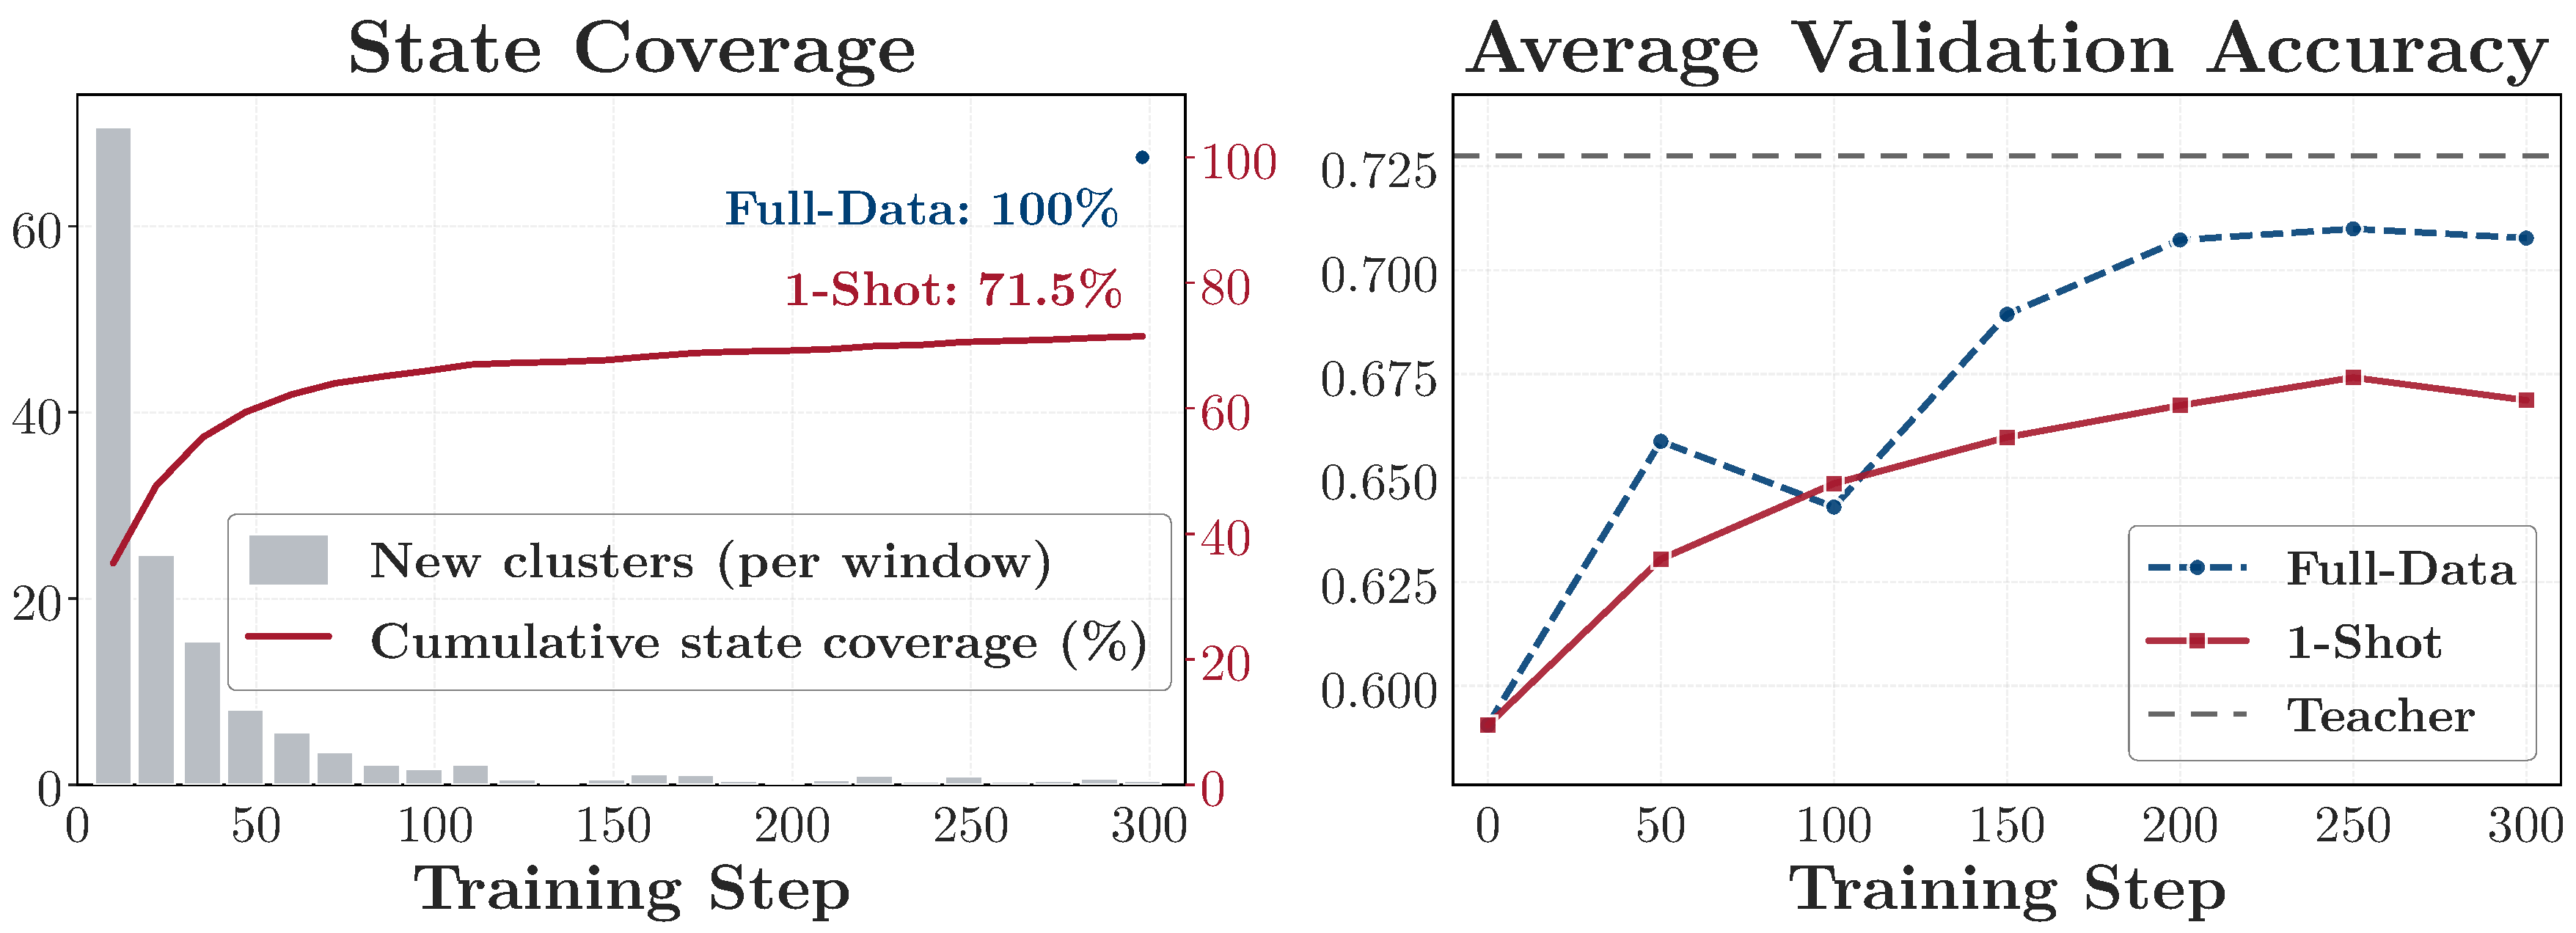
\includegraphics[width=0.75\linewidth]{figures/4_state_coverage_oneshot.pdf}
  \caption{
    one-shot OPD 在中等查询下的状态覆盖与验证准确率，与全数据 OPD 进行对比。覆盖度是相对于全数据 OPD 所能达到的状态空间进行衡量的，因此其水平为 \(1.0\) ，而非分离的曲线。
  }
  \label{fig:state-coverage}
\end{figure}
图~\ref{fig:state-coverage} 显示，one-shot OPD 在步骤 \(300\) 时达到 \(71.5\%\) 状态覆盖。其中大部分覆盖在早期就已出现：该运行在步骤 \(100\) 时达到 \(65.9\%\)，随后在接下来的 \(200\) 步中仅增加了 \(5.6\) 个百分点的覆盖。因此，从同一查询重复展开仍能发现新的簇，但速度显著下降。  
同一运行将验证准确率从 \(59.1\) 提升至 \(66.9\)，而 full-data OPD 在步骤 \(300\) 时仅为 \(70.8\)。这些结果在数据方面也呈现出相同的模式：单次查询已覆盖 full-data OPD 所能达到的大部分状态空间簇，并带来显著的验证性能提升。因此，one-shot OPD 查询次数较少，却能生成广泛的有效监督。

\subsection{多样性扩展状态覆盖}
\label{sec:state-diversity}

上述分析表明，一次查询已能覆盖大部分全数据状态空间，但因果问题仍待澄清：训练表现良好的运行可能只是沿途访问了更多状态，而这些额外状态并未实际发挥作用。因此，我们直接消融状态覆盖，固定其他设置不变，改变训练数据所能达到的不同状态的数量。

\paragraph{设置}
我们从两个方向提升数据多样性，每个方向都有独立的控制机制。
\textbf{(i) 响应多样性（异策略）。} 我们在 one-shot 查询时仅从初始学生中采样一次 \(64\) 轨迹，并保持该样本池固定，从而消除同策略训练中的干扰因素——在同策略训练中，随着学生不断更新，状态会持续变化。嵌套子集保留 \(1\) 、\(4\) 、\(16\) 或全部 \(64\) 条轨迹，并将保留的轨迹重复填充至每个批量大小为 \(64\) 的批次中。所有条件共享相同的查询、批量大小和最优化预算，因此唯一变化的量是不同轨迹的数量，进而影响状态数量。
\textbf{(ii) 查询多样性（同策略）。} 这些实验则改变查询集，且均遵循数学配置。从 one-shot OPD 使用的中等规模查询开始，我们通过使用 BGE-M3~\citep{chen2024bge} 对 DAPO-Math-17K 进行聚类，每种语义簇选取一个代表性查询，构建出 4- 和 16- shot 查询集，确保每次添加到阶梯中的查询与已有查询在语义上均不重复，随后将这些查询集与全数据 OPD 进行对比。
我们报告每次运行的验证准确率，对于同策略运行还报告状态覆盖情况，其中滚动回放指学生在训练过程中实际生成的轨迹。异策略得分在从步骤 \(300\) 到 \(500\) 的五个评估检查点上取平均。在覆盖方面，全数据条形图代表预留的测试集，设定 \(100\%\) 的上限。

\begin{figure}[t]
  \centering
  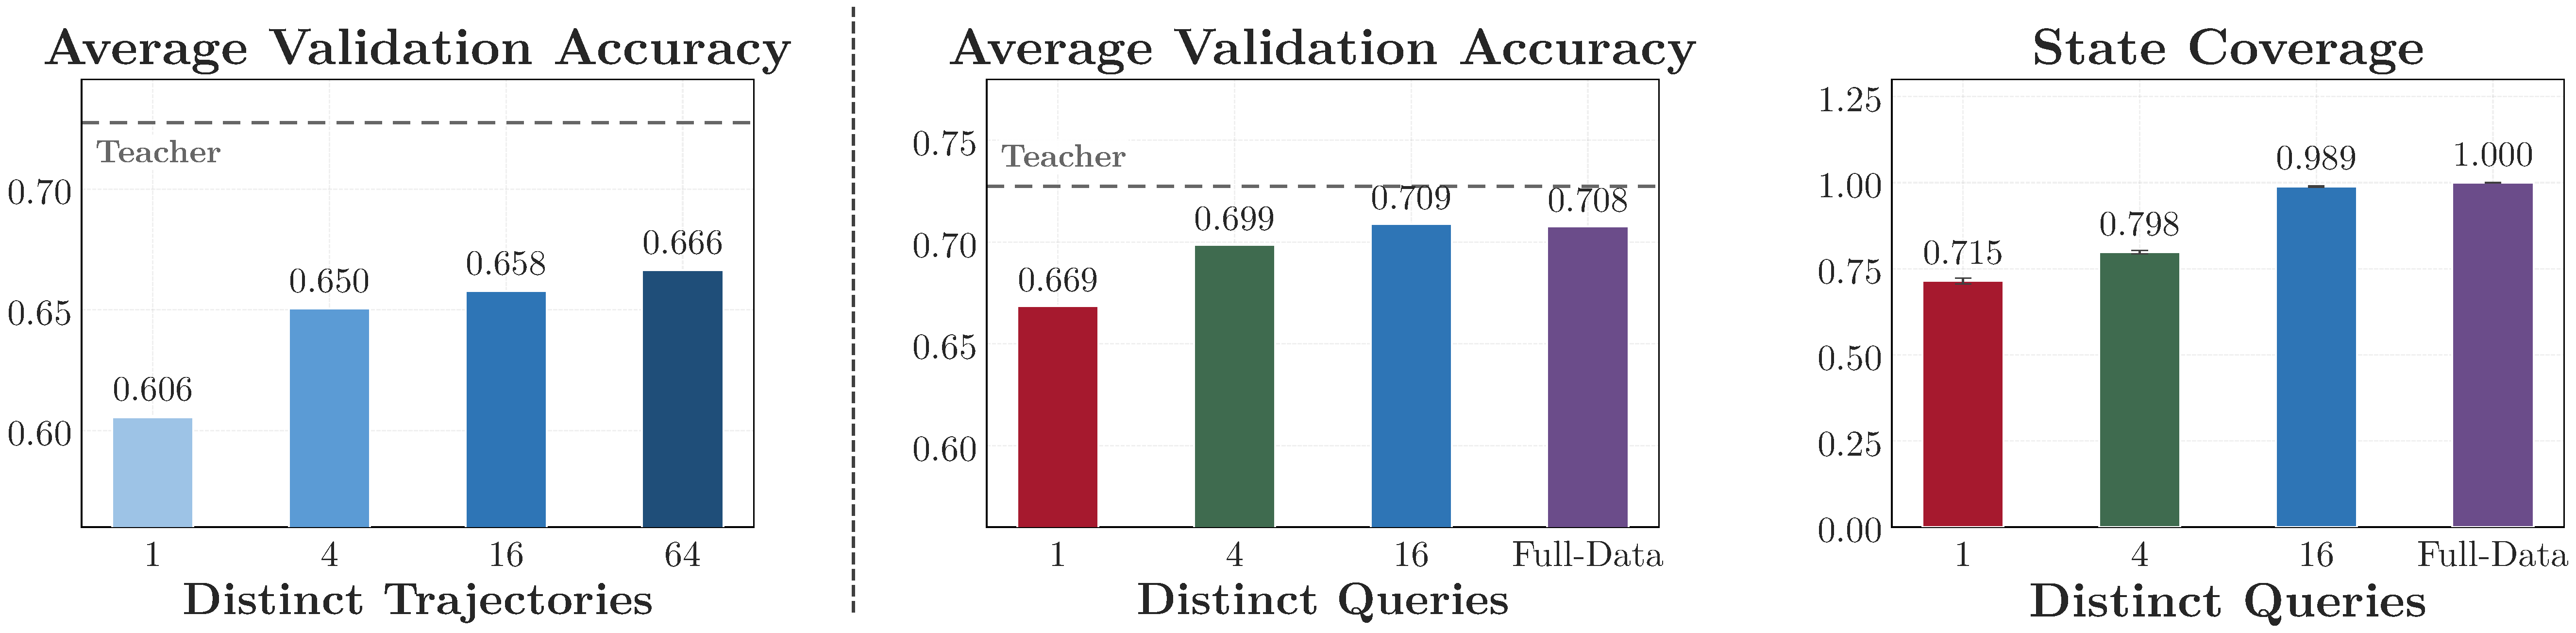
\includegraphics[width=\linewidth]{figures/4_state_diversity.pdf}
    \caption{
    随着训练数据的多样化，验证准确率和状态覆盖情况在响应端通过在不同轨迹上的异策略训练，在查询端通过在不同查询上的同策略训练得到提升。}
  \label{fig:state-diversity}
\end{figure}

\paragraph{数据多样性即状态多样性，少数查询能匹配全数据OPD。}
图~\ref{fig:state-diversity} 显示，随着不同轨迹数量的增加，异策略验证准确率单调上升。其他条件保持不变，因此额外轨迹带来的唯一变化是状态的增加。同策略实验从查询角度得出了相同的结论。语义上不同的查询使验证准确率提升，直到16个查询达到全数据OPD的水平，此时在状态覆盖方面也达到了相同水平，状态覆盖从一个查询时的 \(71.5\%\) 上升至16个查询时的 \(98.9\%\)。梯子上的每一个查询都代表一个新的语义簇，因此同时提升了多样性和数量。附录~\ref{app:fixed-count-diversity} 中的两个控制实验将二者分离：在数量固定为16的情况下，若从16个语义簇中抽取查询而非仅从一个簇中抽取，则状态覆盖和验证准确率会显著提高；而学生在固定查询集上训练的顺序则无关紧要。因此，新增查询的价值取决于其是否能触及新的状态，少数具有多样性的查询已几乎覆盖全数据OPD所能达到的所有状态。